\vspace{-0.1in}
\section{Improved Application Performance in DDC}
\vspace{-0.05in}
\rqc{
Our study so far has focused on characterizing the network requirements for \dis that would lead to little or no performance degradation in existing applications. However, in longer term, one might expect to re-architect existing applications to exploit \dis for improved performance. This is possible due to two factors enabled by \dis: (1) better resource utilization via resource multiplexing{\footnote{As argued in~\cite{hotnets, reiss}, CPU-to-memory utilization for tasks in today’s datacenters varies by three orders of magnitude across tasks. \dis, via statistical multiplexing, enables significantly better resource utilization compared to today's datacenters.}}; and (2) availability of higher density memory architectures~\cite{ddcHwDesign1}.
}

\rc{
While most of the existing applications' performance does not degrade significantly in a DDC, we envision that applications could be rewritten to fully take advantage of disaggregation. 
In COST~\cite{cost}, McSherry et. al. shows that current server centric architecture incurs high overhead to scale out.
For applications such as distributed graph engines, the coordination and communication overhead is too substantial for them to benefit from parallelism.

We conduct a similar experiment as COST~\cite{cost} to show that applications adapted to disaggregated environment can outperform traditional server centric ones.
To simulate an application running in a DDC, we setup a virtual machine with 4 cores and 3GB of memory. 
The server is capable of accessing an ``infinitely'' large remote memory pool by swapping to a RDMA-backed block device. 
We run Pagerank and Connected Components using COST, a single thread graph compute engine over three large graph datasets.
Since COST mmaps the input file, we store the input files into another RDMA-backed block device.
For server centric architecture, we evaluate GraphX using a 16-node m2.4xlarge cluster on EC2. 
Figure \ref{fig:benefit} shows the application runtime of COST-DDC and GraphX-Server Centric.
For most of the case, COST-DDC is 1.48 to 3.04 times faster than GraphX-Server Centric, except Pagerank on UK-2007-5 dataset. 
After talking to one of the author of GraphX, we discovered that the UK-2007-05 dataset has better partition property such that there are fewer vertices spanning machines, hence GraphX performs well. 
We also evaluate the performance benefit of using remote memory over local SSD.
From Figure ~\ref{fig:benefit}, swapping using RDMA is 1.06 to 2.15 times faster than its SSD counterpart. 
}





\vspace{-0.1in}
\section{Related Work and Discussion}
\label{sec:discussion}
\vspace{-0.05in}

As mentioned earlier, there are many recent and ongoing efforts to prototype disaggregated hardware. We discussed the salient features of these efforts inline throughout this paper and hence we only briefly elaborate on them here. 

Lim \etal~\cite{ddcHwDesign1, ddcHwDesign2} discuss the trend of growing peak compute-to-memory ratio, warning of the ``memory capacity wall'' and prototype a disaggregated memory blade. Their results demonstrate that memory disaggregation is feasible and can even provide a 10x performance improvement in memory constrained environments. As noted earlier, our study focuses on the (for us) worst-case scenario where applications are not memory constrained in the non-disaggregated scenario and hence the potential performance degradation due to disaggregation is high. For the same reason, we did not consider redesigning applications to exploit the plentiful remote memory available in \dis. 

Sudan \etal~\cite{ddcHwDesign3} use an ASIC based interconnect fabric to build a virtualized I/O system for better resource sharing. However, these interconnects are designed for their specific context; the authors neither discuss network support for disaggregation more broadly nor consider the possibility of leveraging known datacenter network technologies to enable disaggregation.

Firebox~\cite{firebox} proposes a holistic architecture redesign of datacenter racks to include $1$Tbps silicon phonics links, high-radix switches, remote nonvolatile memory, and System-on-Chips (SoCs). Theia~\cite{theia} proposes a new network topology that interconnects SoCs at high density. Huawei's DC3.0 (NUWA) system uses a proprietary PCIe-based interconnect. R2C2~\cite{r2c2} proposes new topologies, routing and congestion control designs for rack-scale disaggregation.
None of these efforts evaluate network requirements based on existing workloads as we do, nor do they evaluate the effectiveness of existing network designs in supporting disaggregation, or the possibility of disaggregating at scale.

%Overall, we find that related work confirms our prediction that sub-$5\mu$s latencies are feasible in the near future. 

In an early position paper, Han \etal~\cite{hotnets} measure -- as we do -- the impact of remote memory access latency on application-level performance within a single machine. Our work extends this  understanding to a larger set of workloads and concludes with more stringent requirements on latency and bandwidth than Han {\it et al} do, due to our consideration of shark applications. In addition, we use simulation and emulation to study the impact of queueing delay and transport designs which further raises the bar on our target network performance.

%understanding along the new network-oriented design parameters of latency, bandwidth, and transport.Furthermore, our evaluation includes evaluation of additional applications and runs on a cluster of machines ``in the wild,'' measuring realistic scenarios which may have been hidden in a single-machine setting. 

%\paragraphb{Low Latency}
Multiple recent efforts~\cite{farm,mica,herd,ramcloud} aim to reduce the latency in networked applications through techniques that bypass the kernel networking stack, and so forth. %for significant latency improvements with Infiniband RDMA and direct NIC access. 
%Looking forward, CPU-NIC integration, in which the OS kernel and device driver are more directly involved in the low-level operation of the NIC, is on the Simia
Similarly efforts toward NIC integration by CPU architects~\cite{cpu-nic} promise to enable even further latency-saving optimizations. As we note in \S\ref{ssec:rtt}, such efforts are crucial enablers in meeting our latency targets. 










\begin{figure}
  \centering
    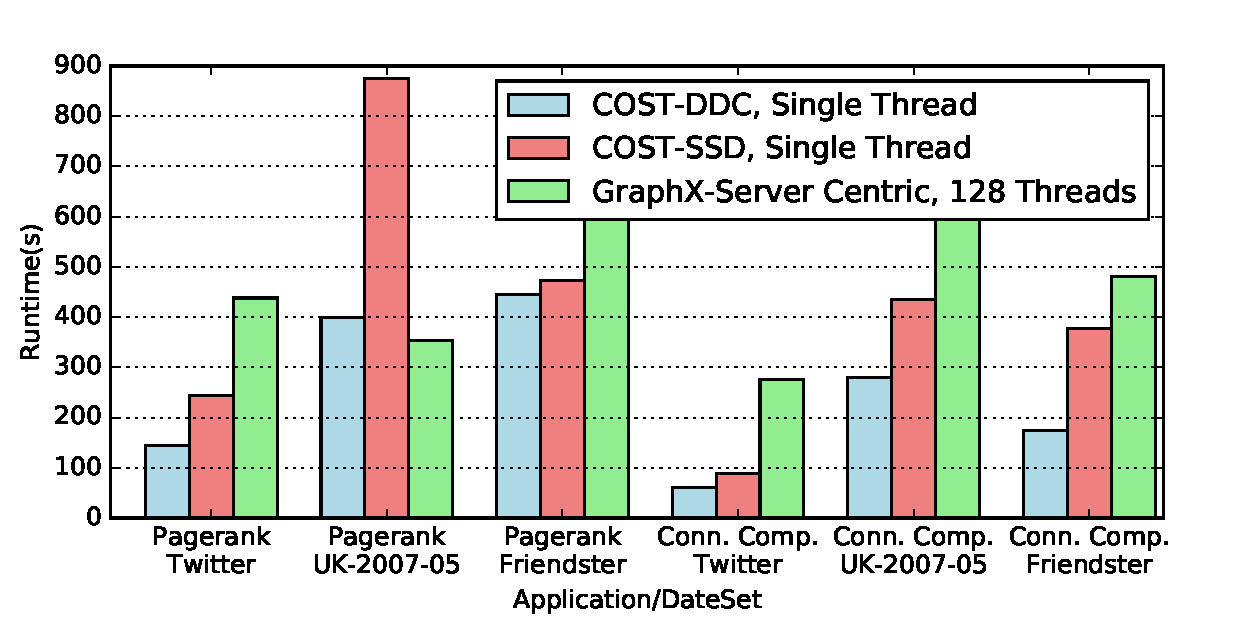
\includegraphics[width = \columnwidth]{img/benefit.eps} 
  \caption{\small{Running COST in a simulated DDC. COST-DDC is 1.48 to 3.04 faster than GraphX-Server Centric. We use three datasets in our evaluation, Twitter (4.17m nodes, 1.47b edges), UK-2007-05 (105m nodes, 3.7b edges), and Friendster (65m nodes, 1.8b edges)}}
  \label{fig:benefit}
\end{figure}







